\documentclass{article}[11pt]
\usepackage{fullpage,graphicx, setspace, latexsym, cite,amsmath,amssymb,xcolor,subfigure}
%\usepackage{epstopdf}
%\DeclareGraphicsExtensions{.pdf,.eps,.png,.jpg,.mps} 
\usepackage{amssymb} %maths
\usepackage{amsmath} %maths
\usepackage{amsthm, comment}
\usepackage[round,comma,sort,numbers]{natbib}

% \bibliographystyle{plain}
\bibliographystyle{plos2015}

\newtheorem{theorem}{Theorem}
\newtheorem{prop}{Proposition}
\newtheorem{corollary}{Corollary}
\newtheorem{lemma}{Lemma}
\newtheorem{defn}{Definition}
\newtheorem{ex}{Example}
\usepackage{float}

\newcommand*{\underuparrow}[1]{\underset{\uparrow}{#1}}
\usepackage{graphicx}
\usepackage{xcolor}
\usepackage[dvipsnames]{xcolor}
\usepackage{algorithmicx}
\usepackage{algorithm} %http://ctan.org/pkg/algorithms
\usepackage{algpseudocode} %http://ctan.org/pkg/algorithmicx
\usepackage{enumitem}
\usepackage{simplemargins}
\usepackage{hyperref}
\hypersetup{
     colorlinks=true,
     linkcolor=blue,
     filecolor=red,
     citecolor = red,      
     urlcolor=cyan,
}

\usepackage{mdframed}
\definecolor{lgray}{rgb}{0.92,0.92,0.92}
\definecolor{lsalmon}{rgb}{0.9921568627450981,0.9411764705882353, 0.9254901960784314}

\renewcommand{\bibnumfmt}[1]{#1.}
\setlist{noitemsep} % or \setlist{noitemsep} to leave space around whole list
\setallmargins{1in}
\linespread{1.1}

\newcommand{\brows}[1]{%
  \begin{bmatrix}
  \begin{array}{@{\protect\rotvert\;}c@{\;\protect\rotvert}}
  #1
  \end{array}
  \end{bmatrix}
}
\newcommand{\rotvert}{\rotatebox[origin=c]{90}{$\vert$}}
\newcommand{\rowsvdots}{\multicolumn{1}{@{}c@{}}{\vdots}}


\def\R{\mathbb{R}}
\def\Eps{\mathcal{E}}
\def\E{\mathbb{E}}
\def\V{\mathbb{V}}
\def\F{\mathcal{F}}
\def\G{\mathcal{G}}
\def\H{\mathcal{H}}
\def\S{\mathcal{S}}
\def\D{\mathcal{D}}
\def\P{\mathbb{P}}
\def\1{\mathbf{1}}
\def\n{\nappa}
\def\h{\mathbf{w}}
\def\v{\mathbf{v}}
\def\x{\mathbf{x}}
\def\X{\mathcal{X}}
\def\Y{\mathcal{Y}}
\def\eps{\epsilon}
\def\y{\mathbf{y}}
\def\e{\mathbf{e}}
\newcommand{\norm}[1]{\left|\left|#1\right|\right|}
\DeclareMathOperator*{\argmin}{arg\,min}
\DeclareMathOperator*{\argmax}{arg\,max}
\newcommand{\lecture}[4]{
   \pagestyle{myheadings}
   \thispagestyle{plain}
   \newpage
   % \setcounter{lecnum}{#1}
   \setcounter{page}{1}
   \setlength{\headsep}{10mm}
   \noindent
   \begin{center}
   \framebox{
      \vbox{\vspace{2mm}
    \hbox to 6.28in { {\bf CHEME 5820: Machine Learning for Engineers
   \hfill Spring 2025} }
       \vspace{4mm}
       \hbox to 6.28in { {\Large \hfill Lecture #1: #2  \hfill} }
       \vspace{2mm}
       \hbox to 6.28in { {\it Lecturer: #3 \hfill #4} }
      \vspace{2mm}}
   }
   \end{center}
   \markboth{Lecture #1: #2}{Lecture #1: #2}

   \noindent{\bf Disclaimer}: {\it These notes have not been subjected to the
   usual scrutiny reserved for formal publications. }
   \vspace*{4mm}
}

\begin{document}
\lecture{5c}{Support Vector Machines (SVMs)}{Jeffrey Varner}{}

\begin{mdframed}[backgroundcolor=lgray]
The key concepts covered in this lecture include:
\begin{itemize}[leftmargin=16pt]
    \item{A \href{sec:svm}{support vector machine} is a supervised machine learning algorithm that finds an optimal hyperplane in an $N$-dimensional space to classify (binary) data points distinctly, maximizing the \textit{margin} between different classes. 
    The \textit{margin} in a support vector machine is defined as the distance from the separating hyperplane to the closest data points of either class.}
    \item{A \href{sec:max-margin}{hard margin support vector machine} is a binary linear classifier that finds the optimal hyperplane to separate two classes of data points with the maximum possible \textit{margin}, allowing no misclassifications and requiring the data to be linearly separable.}
    \item{A \href{sec:soft-margin}{soft margin support vector machine} is a variant of the SVM algorithm that allows for some misclassification of training data points, enabling it to handle non-linearly separable datasets and reduce overfitting by finding a balance between maximizing the decision boundary margin and minimizing classification errors.}
\end{itemize}
\end{mdframed}

\section{Introduction}
In the previous lectures, we've discussed several binary classification algorithms, 
including the perceptron, logistic regression, K-nearest neighbors, and the concept of Kernel functions and the kernel trick.
In this lecture, we will conclude our discussion (for now) of classification algorithms by introducing support vector machines (SVMs). This powerful and versatile machine learning algorithm can be used for classification and regression tasks. 
SVMs are particularly well-suited for binary classification problems, where the goal is to separate data points into two classes using a hyperplane, e.g., like the perceptron.
However, SVMs are based on the concept of finding an \textit{optimal separating hyperplane} (not just some separating hyperplane) 
that maximizes the margin between the two classes. 
Support vector machines are widely used in practice and have been successfully applied to a wide range of applications and problem domains \cite{CERVANTES2020189}, 
such as health care \cite{info15040235}, polymer science \cite{polym17040491}, bioinformatics \cite{Byvatov:2003aa} and understanding the complexity of human decisions \cite{Lamani:2025aa}.

\section{Support Vector Machines (SVMs)}\label{sec:svm}
Support vector machines (SVMs) are a class of supervised learning algorithms that can be used for both classification and regression tasks, 
published by Cortes and Vapnik \cite{Cortes:1995aa} while they worked at AT\&T Bell Labs.
In many ways, SVMs are similar to the perceptron and logistic regression, as they are also based on the concept (in the simplest case) of finding a hyperplane that separates data points into different classes.
Suppose, we have dataset $\mathcal{D} = \{(\hat{\mathbf{x}}_{i}, y_{i}) \mid i = 1,2,\dots,n\}$, where $\hat{\mathbf{x}}_i \in \R^p$ is an \textit{augmented} feature vector ($m$ features with an additional $1$ as the last entry to model the bias) and $y_i \in \{-1, 1\}$ is the corresponding class label.
Then, the goal of SVMs is to find the hyperplane $\mathcal{H} = \{\hat{\mathbf{x}} \mid \left<\hat{\mathbf{x}},\theta\right> = 0\}$ that separates the data points into two classes (those points above the hyperplane, and those points below the hyperplane), 
where $\theta \in \R^{p}$ ($p=m+1$) is the normal vector to the hyperplane, or the parameters of the model that we need to estimate.
So far, this is similar to the perceptron and logistic regression, but the key difference is that SVMs aim to find the \textit{optimal} hyperplane in some sense. 
Let's explore the notion of an \textit{optimal hyperplane} in more detail.


\begin{figure}
    \centering
	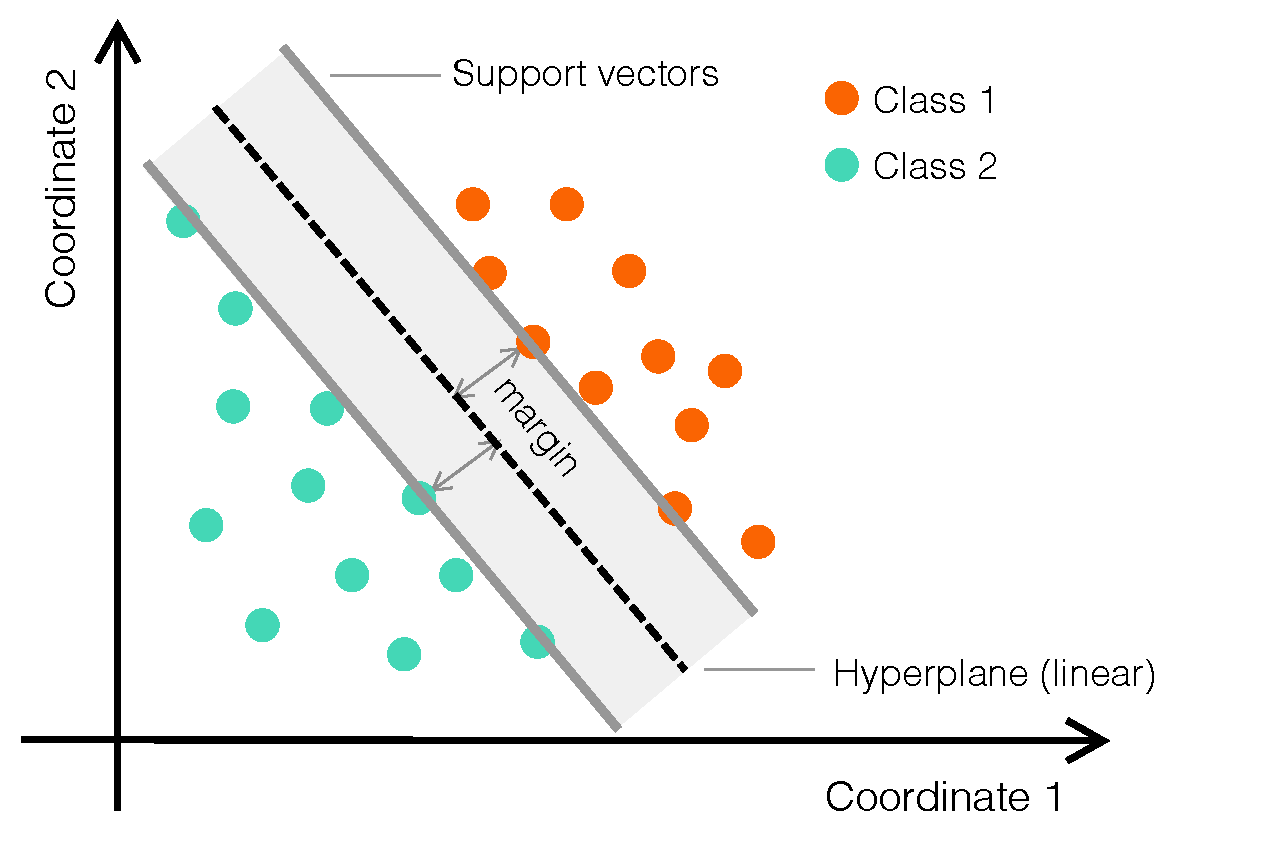
\includegraphics[width=0.64\textwidth]{./figs/Fig-SVM-Schematic.pdf}
	\caption{Schematic of a hard-margin binary classification task with linearly separable data.
    Above the hyperplane are positive examples, while below the hyperplane are negative examples.
    A support vector machine with a hard margin maximizes the width of the gray box, i.e., finds the widest possible
    distance between the hyperplane and the closest data points (of either class) without allowing misclassifications.}\label{fig:linearhyperplane-svm}
\end{figure}

\subsection{Maximum Hard Margin Classifier}\label{sec:max-margin}
Suppose we have found a hyperplane $\mathcal{H}$ that separates the data points into two classes (Fig. \ref{fig:linearhyperplane-svm}).
The margin of the hyperplane is defined as the distance $\gamma$ between the hyperplane and the closest data point from either class.
Thus, the margin measures how well the hyperplane separates the two classes, and the goal of a maximizing margin SVM classifier is to find the hyperplane that maximizes the margin.
Let's develop a model for the margin of the separating hyperplane.

Consider some feature vector $\hat{\mathbf{x}} \in \R^{p}$. Let $\mathbf{d}$ denote the vector from the hyperplane $\mathcal{H}$ to the feature vector $\hat{\mathbf{x}}$.
Finally, let the point $\mathbf{p}$ be the projection of $\hat{\mathbf{x}}$ onto the hyperplane $\mathcal{H}$.
Because the vector $\mathbf{d}$ is orthogonal to the hyperplane $\mathcal{H}$, we can write $\mathbf{d} = \hat{\mathbf{x}} - \mathbf{p}$.
Further, the vector $\mathbf{d}$ can be written as some scalar multiple of the normal vector $\theta$, i.e., $\mathbf{d} = \lambda \theta$, 
where $\theta\in\R^{p}$ is the normal vector to the hyperplane (and the unknown parameters!).
Then we can find the value of $\lambda$ by taking the inner product between $\mathbf{d}$ and the normal vector $\theta$:
\begin{align*}
    \hat{\mathbf{p}} & = \hat{\mathbf{x}} - \mathbf{d}\quad\mid\,\text{take inner product with $\theta$} \\
    \left<\hat{\mathbf{p}},\theta\right> & = \left<\hat{\mathbf{x}},\theta\right> - \left<\mathbf{d},\theta\right> = 0\quad\mid\,\text{substitute $\mathbf{d} = \lambda \theta$} \\
    \left<\hat{\mathbf{p}},\theta\right> & = \left<\hat{\mathbf{x}},\theta\right> - \lambda \left<\theta,\theta\right> = 0\quad\mid\,\text{solve for $\lambda$} \\
    \lambda & = \frac{\left<\hat{\mathbf{x}},\theta\right>}{\left<\theta,\theta\right>}
\end{align*}
We can now find the length of the vector $\mathbf{d}$ by computing the norm $\norm{\mathbf{d}}_{2}$:
\begin{align*}
    \norm{\mathbf{d}}_{2} & = \sqrt{\mathbf{d}^{\top}\mathbf{d}}\quad\mid\,\text{substitute $\mathbf{d} = \lambda \theta$} \\
    & = \sqrt{\lambda^{2}\theta^{\top}\theta}\quad\mid\,\text{substitute $\lambda = \frac{\left<\hat{\mathbf{x}},\theta\right>}{\left<\theta,\theta\right>}$} \\
    & = \sqrt{\frac{\left<\hat{\mathbf{x}},\theta\right>^{2}}{\left<\theta,\theta\right>^{2}}\,\theta^{\top}\theta}\quad\mid\, \text{substitute $\left<\theta,\theta\right> = \theta^{\top}\theta$ and simplify} \\
    & = \frac{\left<\hat{\mathbf{x}},\theta\right>}{\norm{\theta}_{2}}\quad\mid\,\text{where $\norm{\theta}_{2} = \sqrt{\left<\theta,\theta\right>}$}
\end{align*}
The length of the distance vector $\mathbf{d}$ gives us the distance from a feature vector $\hat{\mathbf{x}}$ to the hyperplane $\mathcal{H}$.
Thus, we can define the margin $\gamma_{\theta}$ of the hyperplane $\mathcal{H}$ as the distance between the hyperplane and the closest data point (Defn. \ref{defn:margin}).
\begin{defn}[Margin]\label{defn:margin}
    The margin $\gamma_{\theta}$ of a hyperplane $\mathcal{H}$ is given by the distance between the hyperplane and the closest data point:
    \begin{align*}
        \gamma_{\theta} & = \min_{i}\left\{\frac{|\left<\hat{\mathbf{x}}_{i},\theta\right>|}{\norm{\theta}_{2}}\right\}
    \end{align*}
where we use the absolute value to account for the fact that the distance can be positive or negative, i.e., the data point can be on either side of the hyperplane.
\end{defn}

On interesting feature of the margin is that it is scale-invariant, i.e., the margin is the same regardless of the scale of the normal vector $\theta$
(Lemma \ref{lem:scale-invariance}).
\begin{lemma}[Scale Invariance]\label{lem:scale-invariance}
    The margin $\gamma_{\theta}$ is scale-invariant, i.e., the margin is the same regardless of the normal vector $\theta$ scale.
    To see that the margin is scale-invariant, consider the scaled normal vector $\theta^{\prime} = \alpha\theta$, where the scalar $\alpha\neq{0}$.
    Then, we can show that the margin of the scaled normal vector $\theta^{\prime}$ is the same as the margin of the original normal vector $\theta$:
    \begin{align*}
        \gamma_{\theta^{\prime}} & = \min_{i}\left\{\frac{|\left<\hat{\mathbf{x}}_{i},\theta^{\prime}\right>|}{\norm{\theta^{\prime}}_{2}}\right\}\quad\mid\,\text{substitute $\theta^{\prime} = \alpha\theta$} \\
        & = \min_{i}\left\{\frac{|\left<\hat{\mathbf{x}}_{i},\alpha\theta\right>|}{\norm{\alpha\theta}_{2}}\right\}\quad\mid\,\text{substitute $\norm{\alpha\theta}_{2} = |\alpha|\norm{\theta}_{2}$} \\
        & = \min_{i}\left\{\frac{|\alpha\left<\hat{\mathbf{x}}_{i},\theta\right>|}{|\alpha|\norm{\theta}_{2}}\right\}\quad\mid\,\text{cancel out $\alpha$} \\
        & = \min_{i}\left\{\frac{|\left<\hat{\mathbf{x}}_{i},\theta\right>|}{\norm{\theta}_{2}}\right\} = \gamma_{\theta}
    \end{align*}
    Practically, this means the margin only depends on the direction of the normal vector $\theta$, not its magnitude.
    Thus, we can set the scale to be whatever is most convenient.
\end{lemma}

Now that we have a model for the margin of the hyperplane, we can define the problem of finding the optimal hyperplane as an optimization problem.
Ideally, we would like to estimate the parameters $\theta$ of the hyperplane that maximize the margin $\gamma_{\theta}$, i.e., the distance between the hyperplane and the closest data point is maximized:
\begin{equation*}\label{eq:max-margin}
    \max_{\theta}\gamma_{\theta}\quad\text{subject to}\quad y_{i}\left<\hat{\mathbf{x}}_{i},\theta\right> \geq 0\quad\forall i
\end{equation*}
We can substitute the definition of the margin $\gamma_{\theta}$ into the optimization problem, which gives as a new objective function:
\begin{equation*}
    \max_{\theta}\left[\min_{i}\left\{\frac{|\left<\hat{\mathbf{x}}_{i},\theta\right>|}{\norm{\theta}_{2}}\right\}\right]\quad\text{subject to}\quad y_{i}\left<\hat{\mathbf{x}}_{i},\theta\right> \geq 0\quad\forall i
\end{equation*}
However, we can factor out the norm of the normal vector $\theta$ from the objective function (constant for $i$) and do a scaling trick
where we set the minimum inner product between the parameters and the augmented feature vectors to be 1 (scale invariance from Lemma \ref{lem:scale-invariance}):
\begin{equation*}
    \max_{\theta}\frac{1}{\norm{\theta}_{2}}\underbrace{\left[\min_{i}\left\{|\left<\hat{\mathbf{x}}_{i},\theta\right>|\right\}\right]}_{=1}\quad\text{subject to}\quad y_{i}\left<\hat{\mathbf{x}}_{i},\theta\right> \geq 0\quad\forall i
\end{equation*}
Finally, maximizing the inverse of a function is equivalent to minimizing the function, which simplifies the hard-margin optimization problem to:
\begin{align*}
    \min_{\theta}\quad & \frac{1}{2}\norm{\theta}_{2}^{2}\\
    \text{subject to}\quad & y_{i}\left<\hat{\mathbf{x}}_{i},\theta\right> \geq 0\quad\forall i\\
    & \min_{i}\left\{|\left<\hat{\mathbf{x}}_{i},\theta\right>|\right\} = 1
\end{align*}
However, the last constraint (our scaling trick) is \textbf{hard} to handle.  We can simplify the optimization problem further and get rid of the last constraint 
by modifying the second set of constraints (Defn. \ref{defn:max-margin}):
\begin{mdframed}
\begin{defn}[Maximim Hard Margin Classifier]\label{defn:max-margin}
The maximum hard margin classifier is the solution of the quadratic programming problem:
\begin{align*}
    \min_{\theta}\quad & \frac{1}{2}\norm{\theta}_{2}^{2}\\
    \text{subject to}\quad & y_{i}\left<\hat{\mathbf{x}}_{i},\theta\right> \geq 1\quad\forall i
\end{align*}
where $\theta\in\R^{p}$ denote the unknown parameters that we are trying to estimate,
$\hat{\mathbf{x}}_{i}\in\R^{p}$ are the augmented feature vectors, $y_{i}\in\{-1,1\}$ are the class labels, and $p=m+1$ is the number of parameters, where $m$ is the number of features.
The index $i$ runs over the training examples, i.e., one constraint per training example.
\end{defn}
\end{mdframed}

The maximum margin classifier problem is a quadratic optimization problem with linear constraints; thus, it can be solved using various optimization approaches.
However, a key practical takeaway is that the maximum hard margin classifier will only exist, i.e., find an optimal hyperplane, if the data points are linearly separable.
Finally, support vector machines get their name from the so-called support vectors (Defn. \ref{defn:max-margin-support-vector})
\begin{defn}[Support Vectors]\label{defn:max-margin-support-vector}
The special case where $y_{i}\left<\hat{\mathbf{x}}_{i},\theta\right> = 1$ are called the \textit{support vectors}. 
For the maximum margin classifier, the support vectors are the data points closest to the hyperplane, i.e., the data points defining the margin.
\end{defn}

\begin{figure}
    \centering
	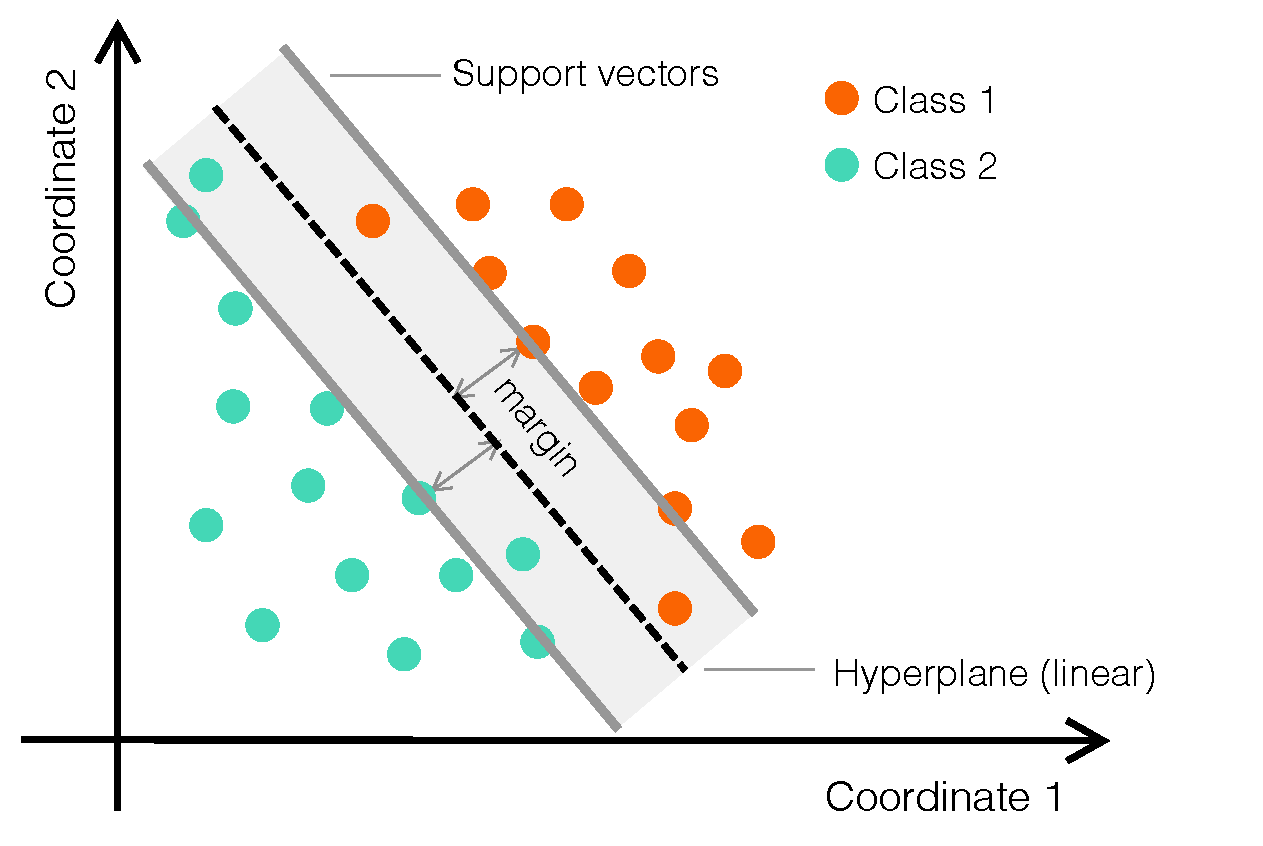
\includegraphics[width=0.64\textwidth]{./figs/Fig-SVM-Schematic-Softmargin.pdf}
	\caption{Schematic of a soft-margin binary classification task with (potentially) non-linearly separable data.
    Above the hyperplane are positive examples, while below the hyperplane are negative examples.
    A support vector machine with a soft margin maximizes the width of the gray box, i.e., finds the widest possible
    distance between the hyperplane and the closest data points (of either class) but will allow points to 
    exist inside the box and will allow misclassifications (at a cost).}\label{fig:linearhyperplane-svm-softmargin}
\end{figure}

\subsection{Soft Margin Classifier}\label{sec:soft-margin}
Suppose there exist points in our dataset $\mathcal{D}$ that are not linearly separable, i.e., there is no hyperplane that can perfectly separate the two classes (Fig. \ref{fig:linearhyperplane-svm-softmargin}).
Just like we did in our perceptron implementation, we can allow the support vector machine to make some mistakes by introducing a slack variable $\xi_{i}$ for each data point.
Let the slack variable $\xi_{i}$ represent the cost of a mistake (in some sense) for the $i$-th data point.
Then, we can modify the constraints and the objective function in the maximum margin classifier problem to allow for some slack, i.e., the constraints are relaxed (Defn. \ref{defn:soft-margin}):
\begin{mdframed}
\begin{defn}[Maximim Soft Margin Classifier]\label{defn:soft-margin}
The soft margin classifier problem is defined as the quadratic programming problem:
\begin{align*}
    \min_{\theta}\quad & \frac{1}{2}\norm{\theta}_{2}^{2} + C\sum_{i=1}^{n}\xi_{i}\\
    \text{subject to}\quad & y_{i}\left<\hat{\mathbf{x}}_{i},\theta\right> \geq 1 - \xi_{i}\quad\forall i\\
    & \xi_{i} \geq 0\quad\forall i
\end{align*}
where $C\geq{0}$ is a user-adjustable parameter that controls the trade-off between maximizing the margin and minimizing the slack variables.
If $C\gg{1}$ the classifier will behave like the maximum margin classifier, and if $C\ll{1}$ the classifier will allow more slack (mistakes).
\end{defn}
\end{mdframed}
We could solve the soft margin classifier problem (directly) using the same optimization techniques as the maximum margin classifier problem.
However, we can also reformulate it as an unconstrained problem by introducing the \texttt{hinge loss} function. 
Let's consider what value the slack variables $\xi_{i}$ can take on (assuming $C>{0}$) where the classifier is correct and when it makes a mistake.
For data points that are correctly classified, the slack variable $\xi_{i}$ will be zero, i.e., $y_{i}\left<\hat{\mathbf{x}}_{i},\theta\right> \geq 1$ 
(The data point is on the correct side of the hyperplane; the SVM didn't make a mistake.) 
However, for misclassified data points, the slack variable $\xi_{i}$ will be positive, i.e., there is a penalty associated with making a mistake. 
Putting these two cases together gives the possible values of the slack variables $\xi_{i}$:
\begin{equation*}
    \xi_{i} = \begin{cases}
        0 & \text{if $y_{i}\left<\hat{\mathbf{x}}_{i},\theta\right> \geq 1$}\,\quad\text{correct}\\
        1 - y_{i}\left<\hat{\mathbf{x}}_{i},\theta\right> & \text{if $y_{i}\left<\hat{\mathbf{x}}_{i},\theta\right> < 1$}\,\quad\text{mistake}
    \end{cases}
\end{equation*}
These two cases can be rewritten in a more convenient form:
\begin{equation*}
    \xi_{i} = \max\{0, 1 - y_{i}\left<\hat{\mathbf{x}}_{i},\theta\right>\}
\end{equation*}
Now we have an expression for the slack variables $\xi_{i}$ in terms of the inner product between the augmented feature vectors and the parameter vector.
We can substitute this expression into the objective function of the soft margin classifier problem, which gives us the \texttt{hinge loss} function (Defn. \ref{defn:hinge-loss}):
\begin{mdframed}
\begin{defn}\label{defn:hinge-loss}
The optimal soft margin classifier problem can be reformulated as an unconstrained optimization problem using the \texttt{hinge loss} function:
\begin{equation*}
    \min_{\theta}\left[\frac{1}{2}\norm{\theta}_{2}^{2} + C\sum_{i=1}^{n}\max\{0, 1 - y_{i}\left<\hat{\mathbf{x}}_{i},\theta\right>\}\right]
\end{equation*}
where $C>{0}$ is a user-adjustable parameter that controls the trade-off between maximizing the margin and minimizing the slack variables.
The hinge loss is not differentiable everywhere, i.e., the gradient is not defined at tie points. 
Thus, we need fancier gradients or alternative techniques such as simulated annealing (or another heuristic method) to solve the problem. 
\end{defn}
\end{mdframed}

\subsection{Kernel SVM}
We will not discuss the underlying theory of the Kernel-SVM in this lecture (instead, we'll build one in lab and see how it works).
However, Kernelized-SVMs handle non-linearly separable data using the kernel trick.
This involves solving the dual optimization problem, which is beyond the scope of this lecture.
For more details on the kernel trick and the dual optimization problem, \href{https://www.cs.cornell.edu/courses/cs4780/2018fa/lectures/lecturenote14.html}{see the CS4780 (2018 fall) lecture 14 notes}. Alternatively, for a much deeper dive, see \href{https://cornell.box.com/s/o2y06fjcjcdsgvqejo434gizc5933qpy}{Chapter 6 of the Ng and Ma CS 229 notes from Stanford University}.


\section{Summary and Conclusions}
In this lecture, we introduced support vector machines (SVMs), a powerful and versatile machine learning algorithm for classification and regression tasks. SVMs are particularly well-suited for binary classification problems, where the goal is to separate data points into two classes using an optimal hyperplane. We also discussed the concept of the maximum margin classifier, which aims to find the hyperplane that maximizes the margin between the two classes. However, the maximum margin classifier only exists if the data points are linearly separable. 
In cases where the data points are not linearly separable, we can use the soft margin classifier, which allows for some slack (mistakes) in the constraints. Finally, we discussed the hinge loss function, which can be used to reformulate the soft margin classifier problem as an unconstrained optimization problem. While not covered in this lecture, SVMs can be extended to handle non-linearly separable data using the kernel trick, which allows us to map the data points into a higher-dimensional space where they are linearly separable. 

\raggedright
\bibliography{References-L5c.bib}

\end{document}


